% !TEX root = ../DuvalPeyre-SparseSpikes.tex

\section{Application to the Ideal Low-pass Filter}
\label{sec-idealLP}

In this section, we apply the results of the previous sections to the particular case of the Dirichlet kernel, defined as
\begin{align}
	\varphi(t) = \sum_{k=-f_c}^{f_c} e^{2i\pi kt} = \frac{\sin \left((2f_c+1)\pi t\right)}{\sin (\pi t)}.
\end{align}


%%%%%%%%%%%%%%%%%%%%%%%%%%%%%%%%%%%%%%%%%%%%%%%%%%%%
\subsection{Elementary Results}

We first check that the assumptions made in Section~\ref{sec-noise-robust} hold in the case of the ideal low-pass filter.


\begin{prop}[Existence of $p_0$]
Let $m\in \Mm(\TT)$ and $y=\Phi m\in L^2(\TT)$. There exists a solution of~\eqref{eq-constrained-dual}.
As a consequence, $p_0\in L^2(\TT)$ is well defined.
\end{prop}

\begin{proof}
We rewrite~\eqref{eq-constrained-dual} as 
\eq{
	\usup{\normi{\eta} \leq 1, \eta \in \Im \Phi^*} \dotp{m}{\eta}.
}
Let $(\eta_n)_{n\in \NN}$ be any maximizing sequence. Then $(\eta_n)_{n\in \NN}$ is bounded in the finite-dimensional space of trigonometric polynomials with degree $f_c$ or less. We may extract a subsequence converging to $\eta^*\in C(\TT)$. But $\normi{\eta^*} \leq 1$ and $\eta^*\in \Im \Phi^*$,
so that $\eta^*=\Phi^*p^*$ for some $p^*$ solution of~\eqref{eq-constrained-dual}.
\end{proof}

\begin{prop}[Injectivity of $\Ga_{x}$]
Let $x=(x_1,\ldots x_N)\in \TT^N$ with $x_i\neq x_j$ for $i\neq j$ and $N\leq f_c$.
Then $\Ga_x=(\Phi_x, \Phi_x')$ has full rank.
\end{prop}

\begin{proof}
Assume that for some $(u,v)\in \RR^N\times \RR^N$, $\Ga_x (u,v)=0$. Then
\begin{align*}
	\foralls  t\in \TT, \quad 0&=\sum_{j=1}^N  \left(u_j\varphi(t-x_j)+v_j \varphi'(t-x_j)\right)\\
&=\sum_{k=-f_c}^{f_c} \left(\sum_{j=1}^N (u_j + 2ik\pi v_j)e^{-2ik\pi x_j}  \right) e^{2ik\pi t}
\end{align*}
We deduce that 
\eq{
	\foralls k\in \{-f_c,\ldots f_c \}, \quad
	\sum_{j=1}^N (u_j + k \tilde{v}_j)r_j^k =0
	\qwhereq
	\choice{
		r_j=e^{-2i\pi x_j},\\
		\tilde{v}_j=2i\pi v_j.
	}
}
It is therefore sufficient to prove that the columns of the following matrix are linearly independent
\begin{align*}
\begin{pmatrix}
r_1^{-f_c} & \ldots &r_N^{-f_c} & (-f_c)r_1^{-f_c}& \ldots &(-f_c)r_N^{-f_c} \\
\vdots & &\vdots  & \vdots & &\vdots \\
r_1^{k} & \ldots &r_N^{k} & kr_1^{k}& \ldots &k r_N^{k} \\
\vdots & &\vdots  & \vdots & &\vdots \\
r_1^{f_c} & \ldots &r_N^{f_c} & (f_c)r_1^{f_c}& \ldots &(f_c)r_N^{f_c} \\
\end{pmatrix}.
\end{align*}
% Since we have not found this result in standard textbooks, we detail the argument.
If $N<f_c$, we complete the family $\{r_1, \ldots r_N\}$ in a family $\{r_0,r_1,\ldots r_{f_c}\}\subset \SS^1$ such
 that the $r_i$'s are pairwise distinct. We obtain a square matrix $M$ by inserting the corresponding columns
\begin{align*}
M = \begin{pmatrix}
r_1^{-f_c} & \ldots &r_{f_c}^{-f_c} & r_0^{-f_c} &(-f_c)r_1^{-f_c}& \ldots &(-f_c)r_{f_c}^{-f_c} \\
\vdots & &\vdots  &\vdots & \vdots & &\vdots \\
r_1^{k} & \ldots &r_{f_c}^{k} & r_0^k &kr_1^{k}& \ldots &k r_{f_c}^{k} \\
\vdots & &\vdots &\vdots & \vdots & &\vdots \\
r_1^{f_c} & \ldots &r_{f_c}^{f_c} & r_0^{f_c}&(f_c)r_1^{f_c}& \ldots &(f_c)r_{f_c}^{f_c} \\
\end{pmatrix}.
\end{align*}
 We claim that $M$ is invertible. Indeed, if there exists $\alpha\in \CC^{(2f_c+1)}$ such that
  $M^T \alpha=0$, then the rational function $F(z) = \sum_{k=-f_c}^{f_c} \alpha_k z^{k}$ satisfies:
\begin{align*}
  	F(r_j)&=0 \qandq F'(r_j)=0 \ \mbox{ for } 1\leq j \leq f_c,\\
  	F(r_0)&=0.
\end{align*}
Hence, $F$ has at least $2f_c+1$ roots in $\SS^1$, counting the multiplicities. This imposes that $F=0$, thus $\alpha=0$,
 and $M$ is invertible. The result is proved.
\end{proof}

%%%%%%%%%%%%%%%%%%%%%%%%%%%%%%%%%%%%%%%%%%%%%%%%%%%%%%%%%%%%%%%
\subsection{Identifiable Measures}

In~\cite{Candes-toward}, Cand\`es and Fernandez-Granda have proved that discrete
 measures are identifiable provided that their support is separated enough, i.e. $\Delta(m) \geq \frac{C}{f_c}$ for some $C>0$, where $\Delta(m)$ is the so-called minimum separation distance.

\begin{defn}[Minimum separation]
The minimum separation of the support of a discrete measure $m$ is defined as
\eq{
 	\Delta(m)=\inf_{(t,t')\in \supp (m)} |t-t'|,
}
where $|t-t'|$ is the distance on the torus between $t$ and $t'\in \TT$, and we assume $t\neq t'$.
\end{defn}

In~\cite{Candes-toward} it is proved that $C \leq 2$ for complex measures (i.e. of the form $m_{a,x}$ for $a \in \CC^N$ and $x \in \TT^N$) and $C \leq 1.87$ for real measures (i.e. of the form $m_{a,x}$ for $a \in \RR^N$ and $x \in \TT^N$). Extrapolating from numerical simulations on a finite grid, the authors conjecture that for complex measures, one has $C\geq 1$. In this section we show that for real measures, necessarily $C\geq \frac{1}{2}$.


% Since real measures seem easier to reconstruct than complex measures, and this conjecture being based on building adversarial complex signals, a smaller constant $C$ might be sufficient for real measures. In this section, we prove that for real measures, we must have $C\geq \frac{1}{2}$.

We rely on the following theorem, proved by P. Tur\'an~\cite{Turan1946}.

\begin{thm}[Tur\'an]
Let $P(z)$ be a non trivial polynomial of degree $n$ such that $|P(1)|=\max_{|z|=1} |P(z)|$. Then for any root $z_0$ of $P$ on the unit circle, $|\arg (z_0)|\geq \frac{2\pi}{n}$. Moreover, if $|\arg (z_0)|= \frac{2\pi}{n}$, then $P(z)=c(1+z)^n$ for some $c\in \CC^*$.
 \label{thm-turan}
\end{thm}

From this theorem we derive necessary conditions for measure that can be reconstructed by~\eqref{eq-constrained-pbm}.

\begin{cor}[Non identifiable measures]
Let $\theta\in (0,\frac{1}{2}]$. Then there exists a discrete measure $m$ with $\Delta(m)=\frac{\theta}{f_c}$ such that $m$ is not a solution of~\eqref{eq-constrained-pbm} for $y=\Phi m$.
\end{cor}

\begin{proof}
Let $m=\delta_{-\theta/f_c}+\delta_{0} - \delta_{\theta/f_c}$. By contradiction, assume that $m$ is a solution to ~\eqref{eq-constrained-pbm},
 and let $\eta\in C(\TT)$ be an associated solution of~\eqref{eq-constrained-dual} (which
  exists since $\Im \Phi^*$ is finite-dimensional).
Then necessarily $\eta(0)=1$ and $\eta(\theta/f_c)=-1$.
The real trigonometric polynomial $D(t)=\frac{1+\eta(t)}{2}$ is non-negative,
 $D(0)=1=\normi{D}$ and $D(\theta/f_c)=0$. If $D(t)=\sum_{k=-f_c}^{f_c}d_k e^{2i\pi kt}$,
  the polynomial $P(z) = \sum_{k=0}^{2f_c}d_{k-f_c}z^k$ satisfies $P(1)=1=\sup_{|z|=1}|P(z)|$,
   and $P(e^{2i\pi\frac{\theta}{f_c}})=0$.
   
If $\theta<\frac{1}{2}$ this contradicts Theorem~\ref{thm-turan}. If $\theta=\frac{1}{2}$,
 then Theorem~\ref{thm-turan} asserts that $P(z)=c(1+z)^{2f_c}$, and from $P(1)=1$ we get $c=\frac{1}{2^{2f_c}}$,
 so that 
 \begin{align*}
 D(t)=e^{-2i\pi f_c}P(e^{2i\pi t})=\left(\cos (\pi f_c t)\right)^{2f_c}.
 \end{align*}
 Then $D(-\frac{\theta}{f_c})=0$, which contradicts the optimality of $\eta$.
As a conclusion, $m$ is not a solution of~\eqref{eq-constrained-pbm}. 
\end{proof}

In a similar way, we may also deduce the following corollary.

\begin{cor}
Let $\tilde{m}_\la=m_{\tilde{a}_\la,\tilde{x}_\la}$ be a discrete solution of Problem $\Pp_\la(y+w)$ where $y=\Phi m$ for any data $m\in \Mm(\TT)$ and any noise $w\in L^2(\TT)$. Let $(\tilde{x}_{\la,i}, \tilde{x}_{\la,j}) \in \supp (m_\la)^2$. If $|\tilde{x}_{\la,i}-\tilde{x}_{\la,j}|\leq \frac{0.5}{f_c}$
then $\sign (\tilde{a}_{\la,j})=\sign (\tilde{a}_{\la,i})$.
\end{cor}

%%%%%%%%%%%%%%%%%%%%%%%%%%%%%%%%%%%%%%%%%%%%%%%%%%%%%%%%%%%%%%%
\subsection{Performance of Pre-certificates}

In order to prove their identifiability result for measures, the authors of~\cite{Candes-toward} introduce a ``good candidate'' for a dual certificate associate to $m=m_{a,x}$ for $a \in \CC^N$ and $x \in \RR^N$. 
For $K$ being the square of the Fejer kernel, they build a trigonometric polynomial
\eq{
	\hat \eta_0(t)=\sum_{i=1}^N \left(\alpha_{i}K(t-x_i) + \beta_{i}K'(t-x_i) \right) \mbox{ with } K(t)=\left(\frac{\sin \left(\left(\frac{f_c}{2}+1 \right)\pi t\right)}{\left(\frac{f_c}{2}+1\right)\sin \pi t}\right)^4
}
and compute $(\al_i,\be_i)_{i=1}^N$ by imposing that $\hat \eta_0(x_i)=\sign (a_i)$ and $\hat \eta_0'(x_i)=0$.

They show that the constructed ``pre-certificate'' is indeed a certificate,  i.e. that $\normi{\hat \eta} \leq 1$, provided that the support is separated enough (i.e. when $\Delta(m)\geq C/f_c$). This results is important since it proves that measures that have sufficiently separated spikes are identifiable. Furthermore, using the fact that $\hat \eta_0$ is not degenerate (i.e. $\hat \eta_0(x_i)'' \neq 0$ for all $i=1,\ldots,N$), the same authors derive  an $L^2$ robustness to noise result in~\cite{Candes-superresol-noisy}, and Fernandez-Granda and Azais et al.  use the constructed certificate to analyze finely the positions of the spikes in~\cite{Fernandez-Granda-support,Azais-inaccurate}.
  
  


From a numerical perspective, we have investigated how this pre-certificate compares with the vanishing derivative pre-certificate that appears naturally in our analysis, by generating random real-valued measures for different separation distances and observing  when each pre-certificate satisfies $\normi{\eta} \leq 1$.


\begin{figure}[ht]
\centering
	\begin{tabular}{@{}c@{\hspace{1mm}}c@{}}
	   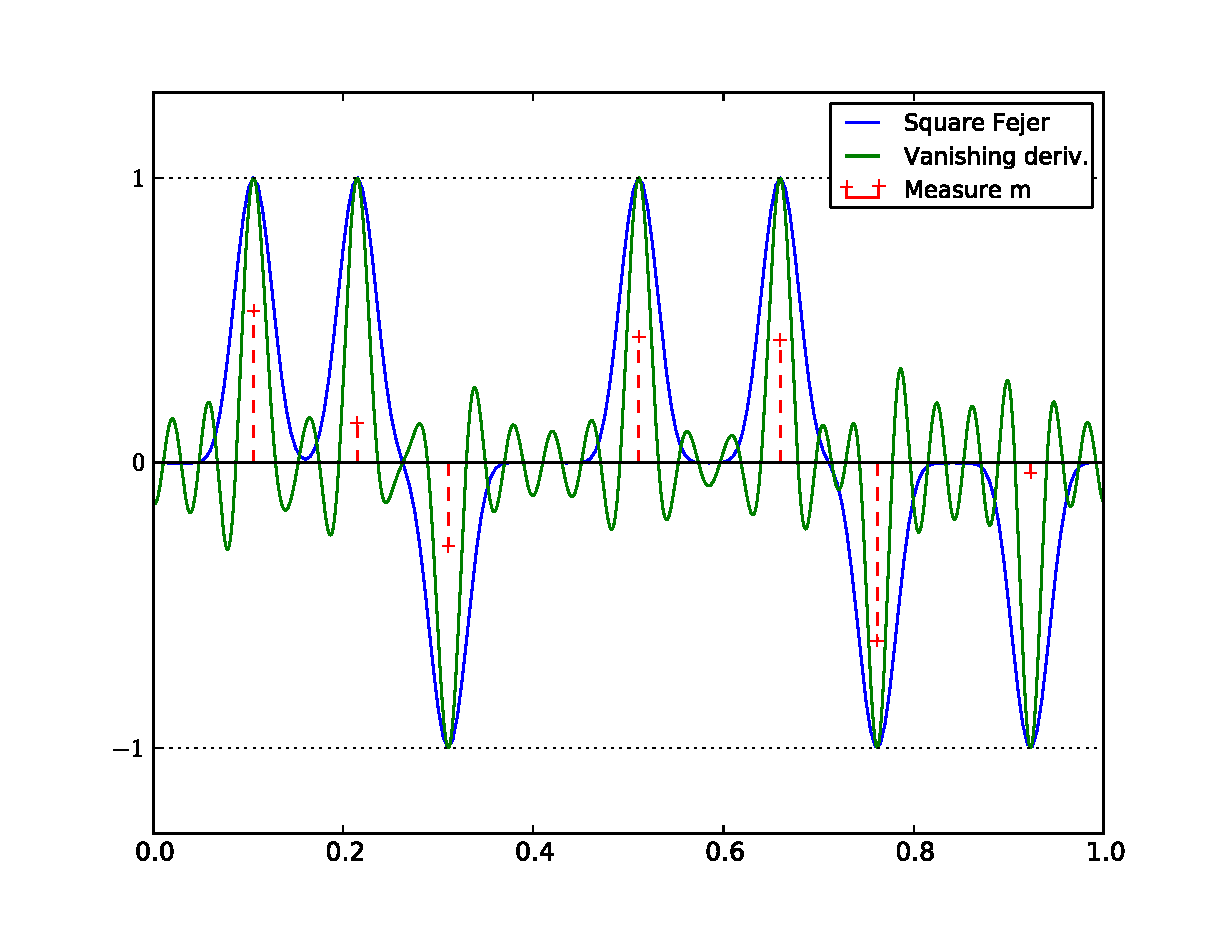
\includegraphics[width=0.46\linewidth] {precertif-2p5.pdf} &
   		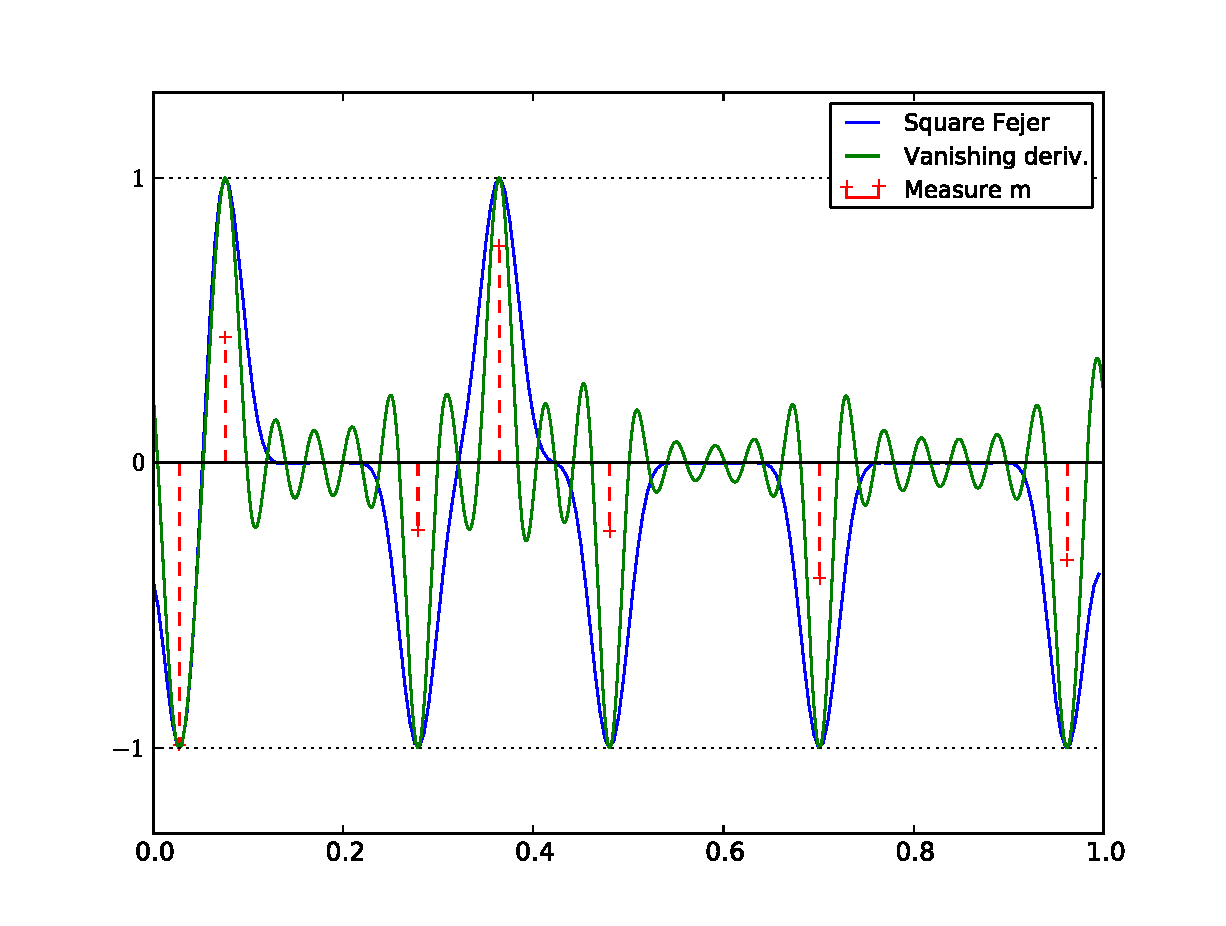
\includegraphics[width=0.46\linewidth] {precertif-1p26.pdf} \\
		$\Delta(m)\approx 2.50/f_c$ & $\Delta(m)\approx 1.26/f_c$ \\[3mm]
	   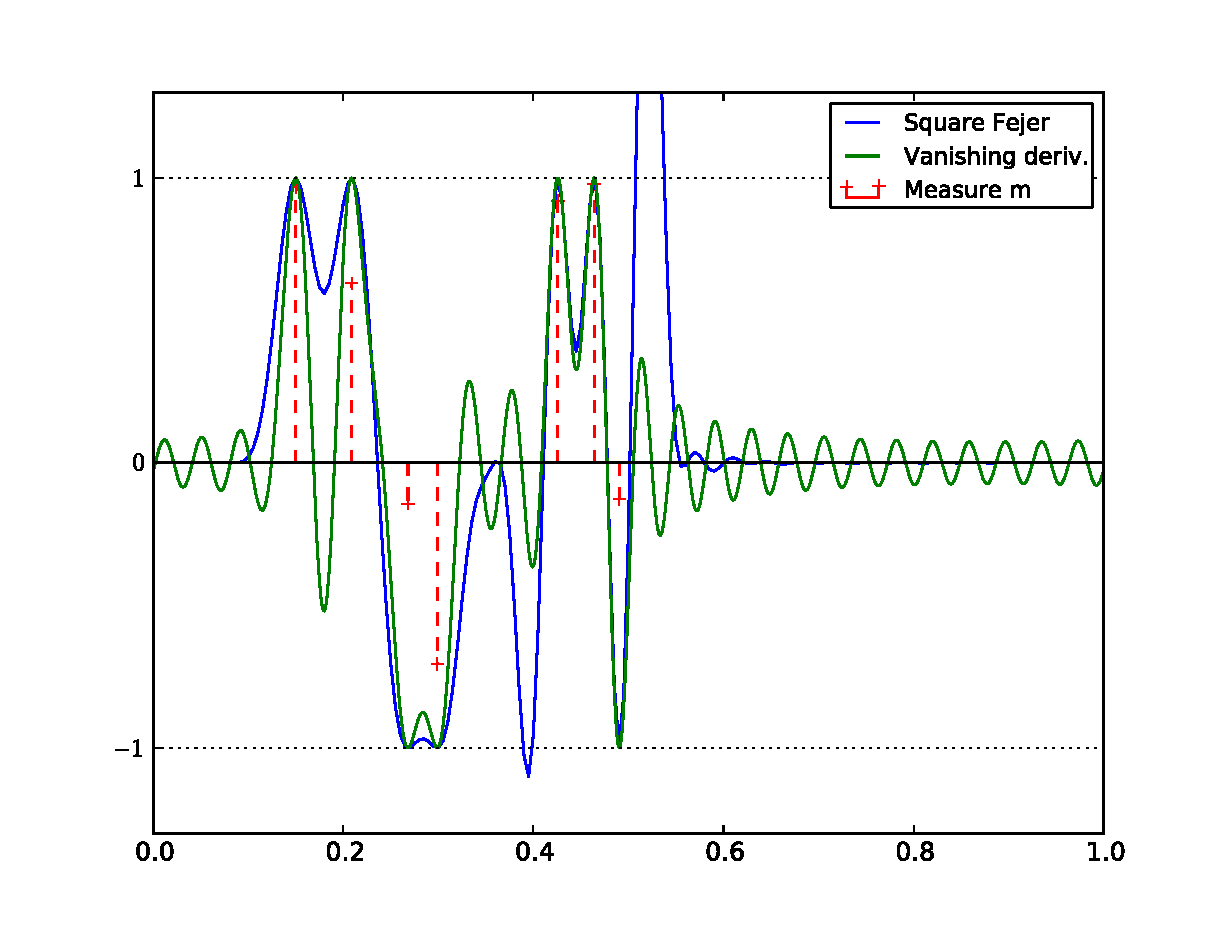
\includegraphics[width=0.46\linewidth] {precertif-0p69.pdf} &
	   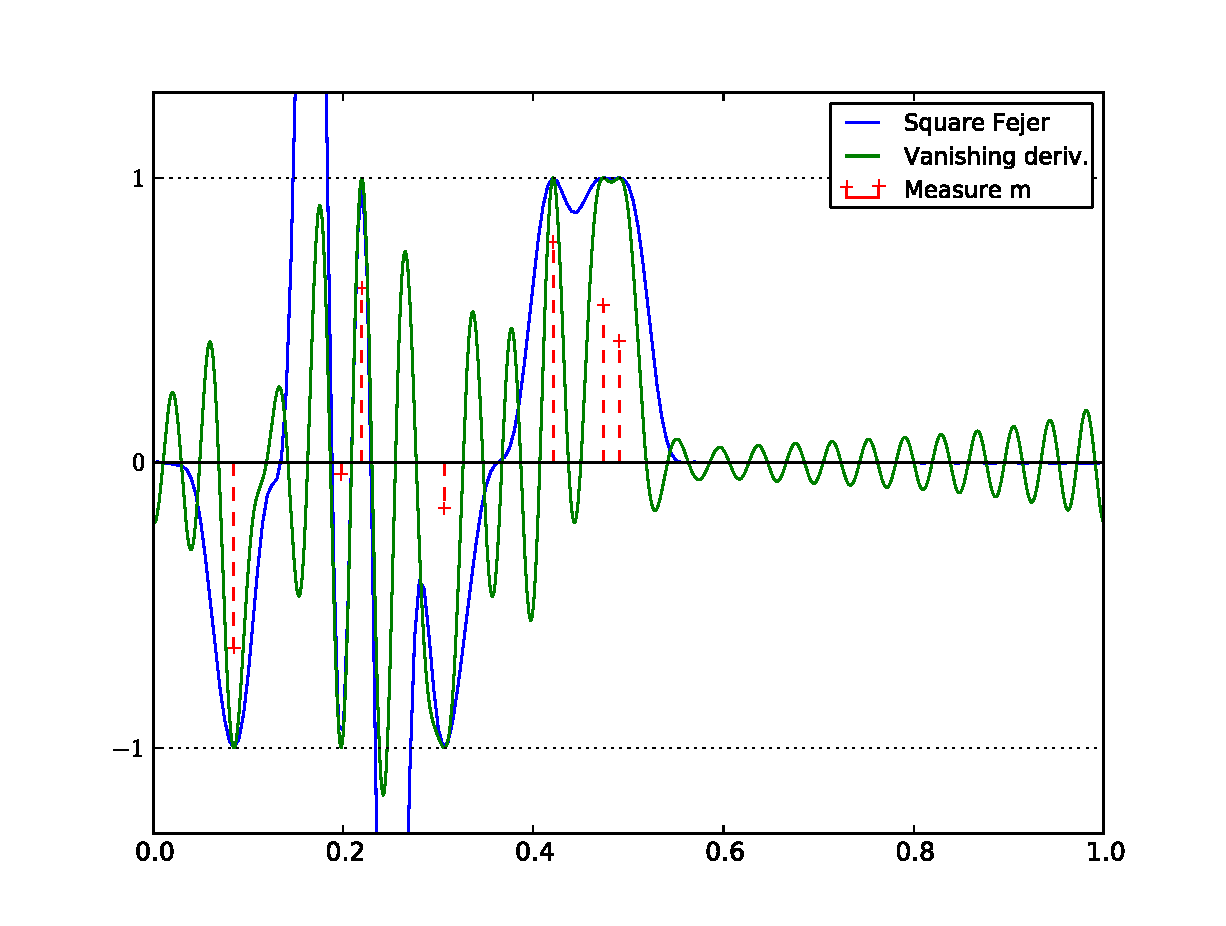
\includegraphics[width=0.46\linewidth] {precertif-0p44.pdf}\\
		$\Delta(m)\approx 0.69/f_c$ & $\Delta(m)\approx 0.44/f_c$
	\end{tabular}
\caption{\label{fig-precertif} % 
The blue curve is the square Fejer kernel pre-certificate $\hat \eta_0$ (introduced in~\cite{Candes-toward}) and the green curve shows the vanishing derivative pre-certificate $\bar\eta_0$, defined in~\eqref{eq-vanishing-der-certif}, for several measures $m$ (whose Diracs' locations and elevation are display in dashed red) with different separation distances $\De(m)$. Eventually when $\Delta(m)$ is small enough, both pre-certificates break (i.e. are not anymore certificates), but the square Fejer always breaks before the vanishing derivative pre-certificate.\vspace{2mm}}
\end{figure}

As predicted by the result of~\cite{Candes-toward}, we observe numerically that the pre-certificate $\hat \eta_0$ is a a certificate (i.e. $\normi{\hat \eta_0} \leq 1$) for any measure with $\De(m) \geq 1.87/f_c$. We also observe that this continues to hold up to $\De(m) \geq 1/f_c$. Yet, below $1/f_c$, we observe numerically that some measures are still identifiable (as asserted using the vanishing derivative pre-certificate $\bar \eta_0$)  but $\hat \eta_0$ stops being a certificate, i.e. $\normi{\hat \eta_0} > 1$. An illustration is given in Figure~\ref{fig-precertif}, where the chosen parameters are $f_c=26$ and $N=7$. For the cases $\Delta(m)=2.50/f_c$ and $\Delta(m)=1.26/f_c$, both pre-certificates $\bar\eta_0$ and $\hat\eta_0$ are certificates, showing that the generated measure is identifiable. Notice how the vanishing derivative certificate $\bar\eta_0$ oscillates much more than the square Fejer certificate $\hat\eta_0$ . For $\Delta(m)=0.69/f_c$, the square Fejer pre-certificate breaks the constraint ($\normi{\eta} \approx 2.39$) whereas the vanishing derivative certificate still satisfies $\normi{\eta} \leq 1$. Eventually, for $\Delta(m)=0.44/f_c$, both pre-certificates violate the constraint, with $\normi{\hat\eta_0} \approx 3.39$ and $\normi{\bar\eta_0}=1.17$ respectively. 
 

In all the experiments that we have led, the vanishing derivative pre-certificate behaved at least as well as the square Fejer. We are not able to prove rigorously this observation, but several facts advocate for this:
\begin{itemize}
 	\item Whenever the square Fejer pre-certificate works, $m$ is a solution of~\eqref{eq-constrained-pbm}, and the minimal norm certificate $\eta_0$
 is then associated to $m$.
 
 	\item Provided that  $|\eta_0| <1$ on $\TT\setminus \supp (m)$ and that $\eta_0''(x_i)\neq 0$
  for all $1\leq i\leq N$, Proposition~\ref{prop-vanish-certif} implies that the
   vanishing derivative pre-certificate $\bar\eta_0$ is equal to $\eta_0$.

	\item It the minimum separation condition holds, the authors of~\cite{Candes-toward} have proved that 
$|\hat \eta_0| <1$ on $\TT\setminus \supp (m)$ and $\hat \eta_0''(x_i)\neq 0$.
\end{itemize}
Intuitively it seems very unlikely that the minimal norm certificate should fail to satisfy $|\eta_0| <1$ on $\TT\setminus \supp (m)$ and $\eta_0''(x_i)\neq 0$ whereas the  square Fejer certificate does not. Indeed the failure of any of those conditions tend to impose a large $L^2$ norm on the considered pre-certificate $\eta$ (recall that when $\phi$ is an ideal low pass filter $\norm{\eta}_2=\norm{p}_2$).
 
 
 
 